\section{Cải tiến về Software}
    So với phiên bản nguyên mẫu vốn chỉ tập trung vào PC App hỗ trợ cấu hình WAN và các giao tiếp LAN cơ bản (LoRa, CAN, RS485), phần mềm cấu hình phiên bản 1.0.0 (DATN\_config\_app) đã được mô-đun hóa mạnh mẽ để đồng bộ với kiến trúc firmware mới. Bên cạnh việc duy trì hai chế độ Basic và Advanced, phiên bản 1.0.0 mở rộng thêm các nhánh cấu hình chuyên sâu cho BLE, BLE Native, Zigbee và chuẩn hóa toàn bộ quy trình qua cơ chế dữ liệu JSON. Sự chuyển đổi này giúp thay thế các lệnh rời rạc bằng một hệ thống quản lý module thống nhất, nâng cao khả năng can thiệp và mở rộng linh hoạt cho hệ thống Gateway.
    % \newpage
    \begin{figure}[h]
        \centering
        \begin{subfigure}[b]{0.48\textwidth}
            \centering
            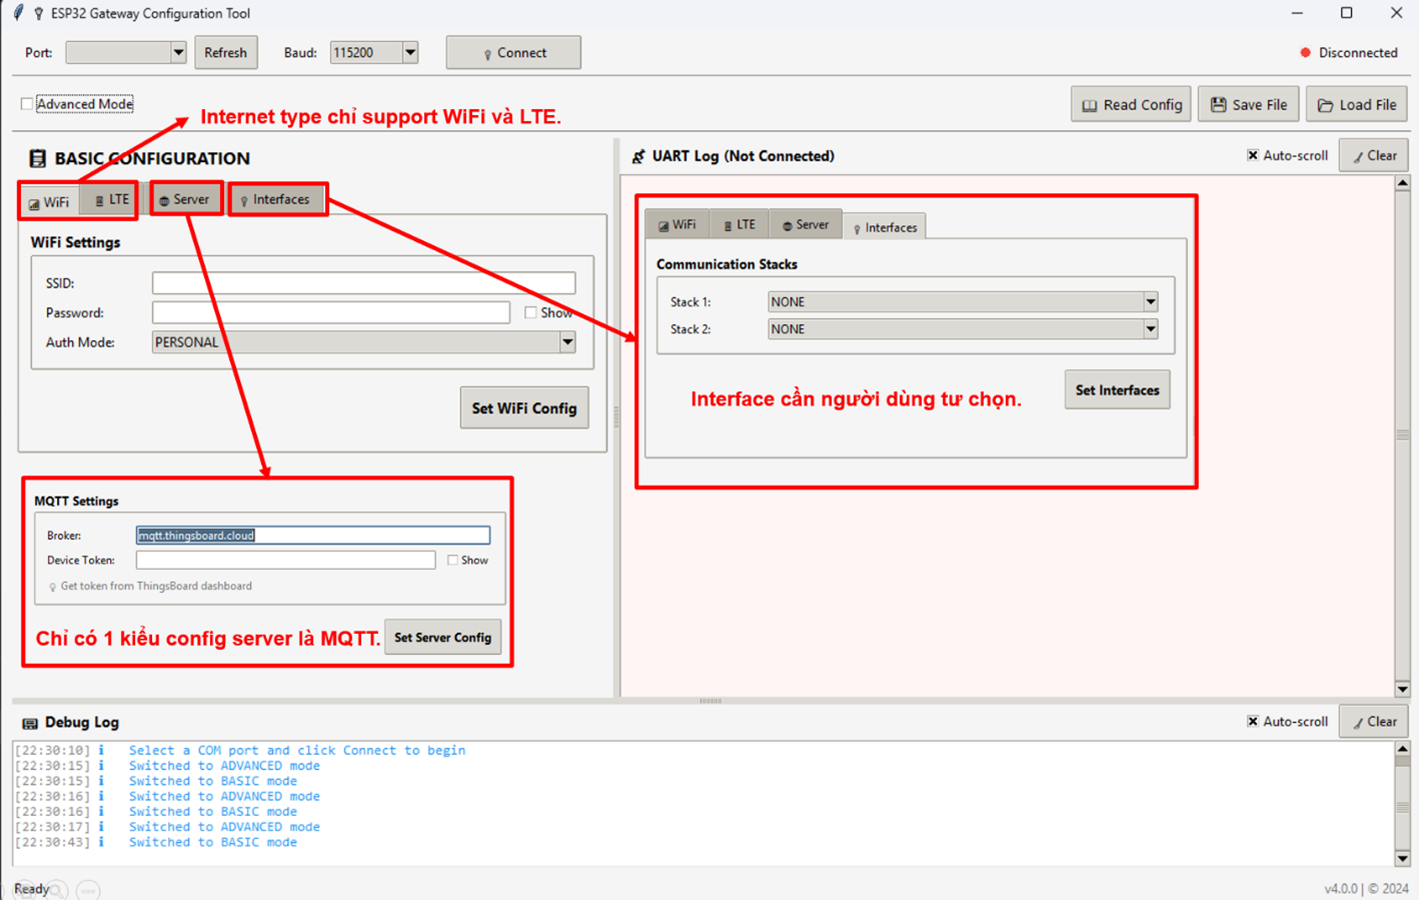
\includegraphics[width=\textwidth]{figures/giao_dien_pc_app_ver_prototype.png}
            \caption{Giao diện cấu hình của PC App phiên bản nguyên mẫu}
        \end{subfigure}
        % \hfill
        \begin{subfigure}[b]{0.48\textwidth}
            \centering
            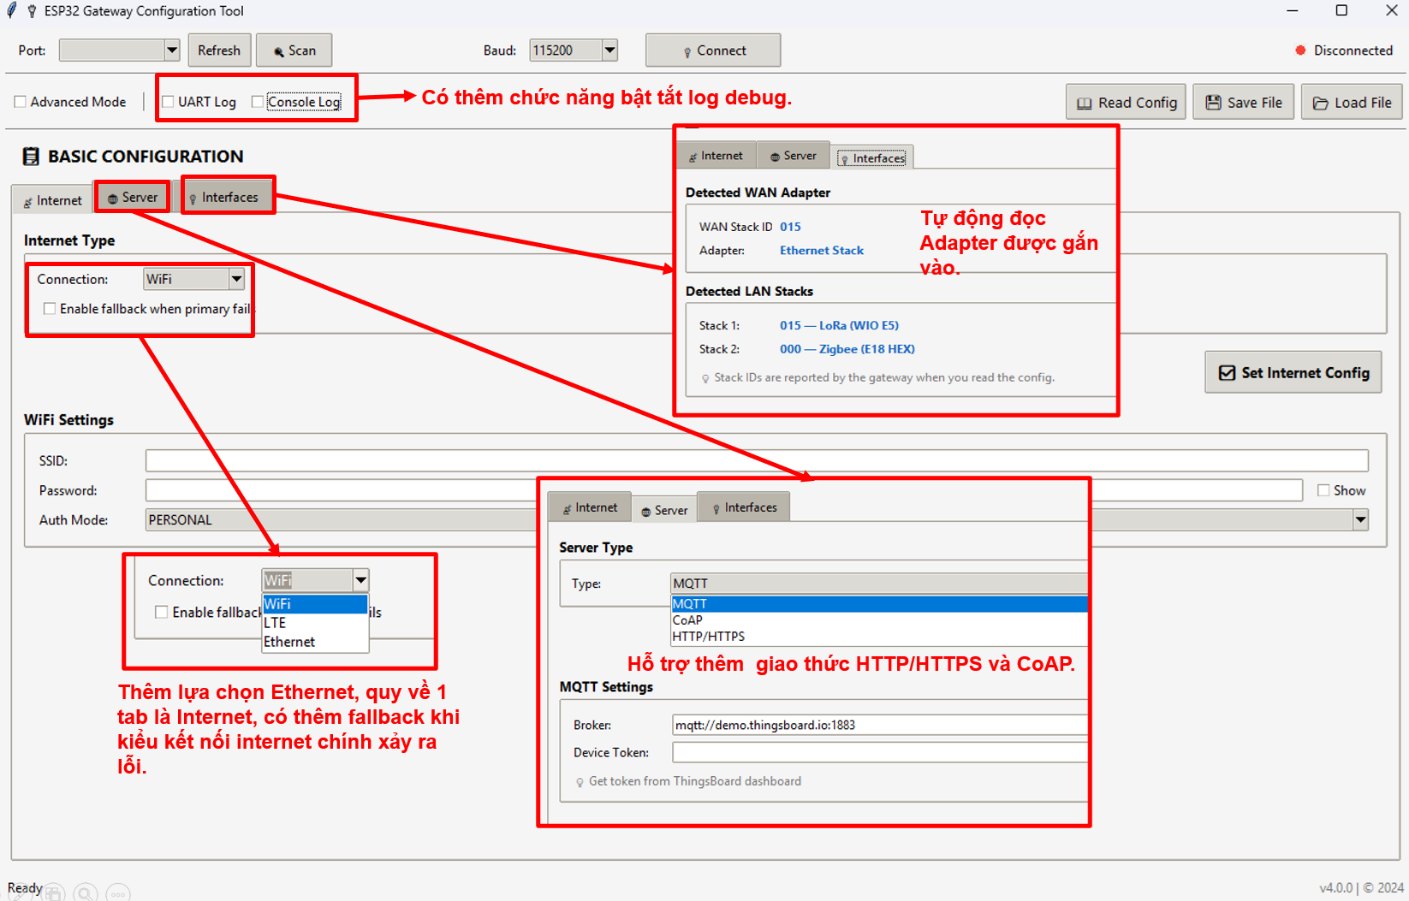
\includegraphics[width=\textwidth]{figures/giao_dien_pc_app_ver_1_0_0.png}
            \caption{Giao diện cấu hình của PC App phiên bản 1.0.0}
        \end{subfigure}
        \caption{So sánh giao diện cấu hình giữa phiên bản nguyên mẫu và phiên bản 1.0.0}
    \end{figure}

    Thay vì gắn chặt logic cấu hình vào mã nguồn và lệnh gửi trực tiếp như phiên bản nguyên mẫu, phiên bản 1.0.0 chuyển sang quản lý tập trung bằng các file JSON preset theo từng stack module. Cải tiến này cho phép cập nhật linh hoạt tập lệnh AT, timeout hay điều khiển GPIO thông qua các file ánh xạ và cấu hình ngoài mà không cần can thiệp vào mã nguồn ứng dụng. Sự cải tiến này không chỉ đồng bộ hóa phần mềm với kiến trúc module setting của firmware mà còn tối ưu hóa khả năng bảo trì và tùy biến hệ thống.
    \begin{figure}[h]
        \centering
        \begin{subfigure}[b]{0.48\textwidth}
            \centering
            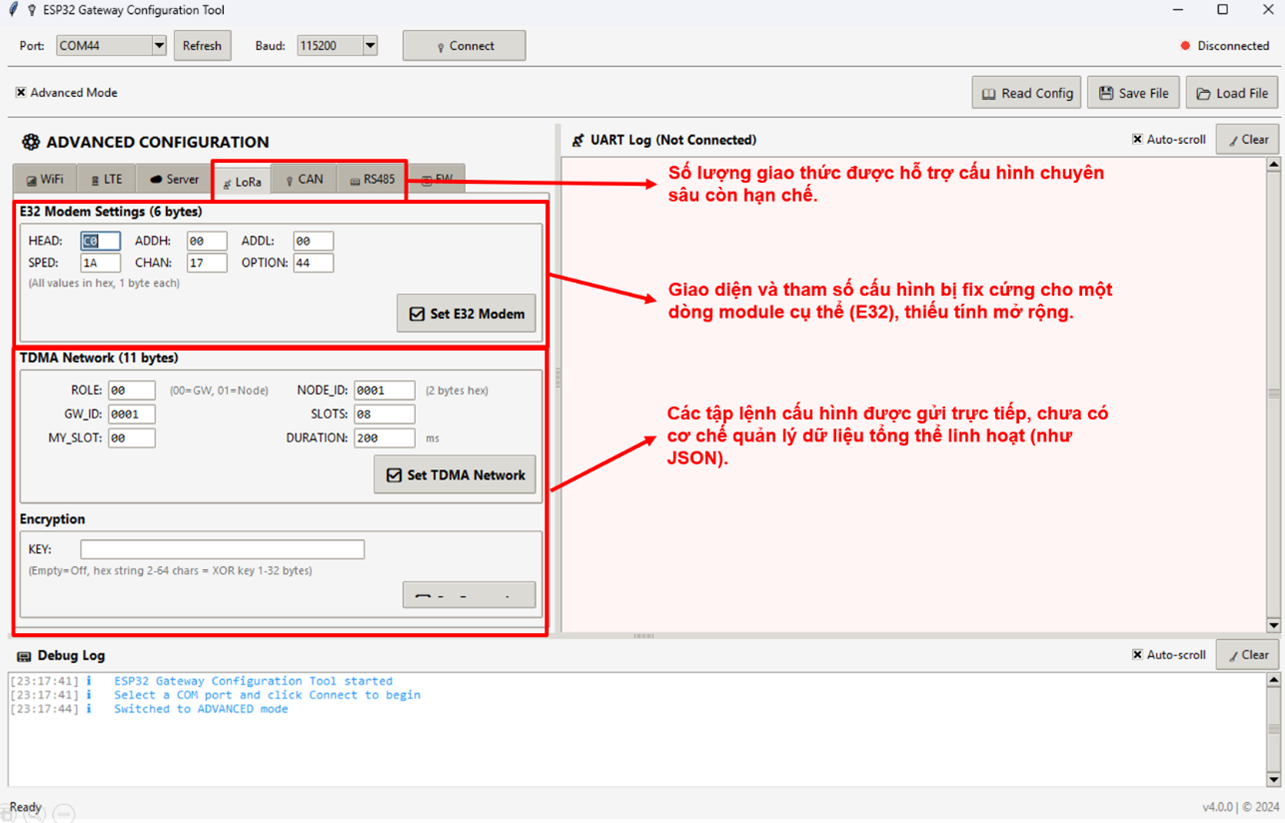
\includegraphics[width=\textwidth]{figures/giao_dien_pc_app2_ver_prototype.png}
            \caption{Logic cấu hình của phiên bản nguyên mẫu}
        \end{subfigure}
        % \hfill
        \begin{subfigure}[b]{0.48\textwidth}
            \centering
            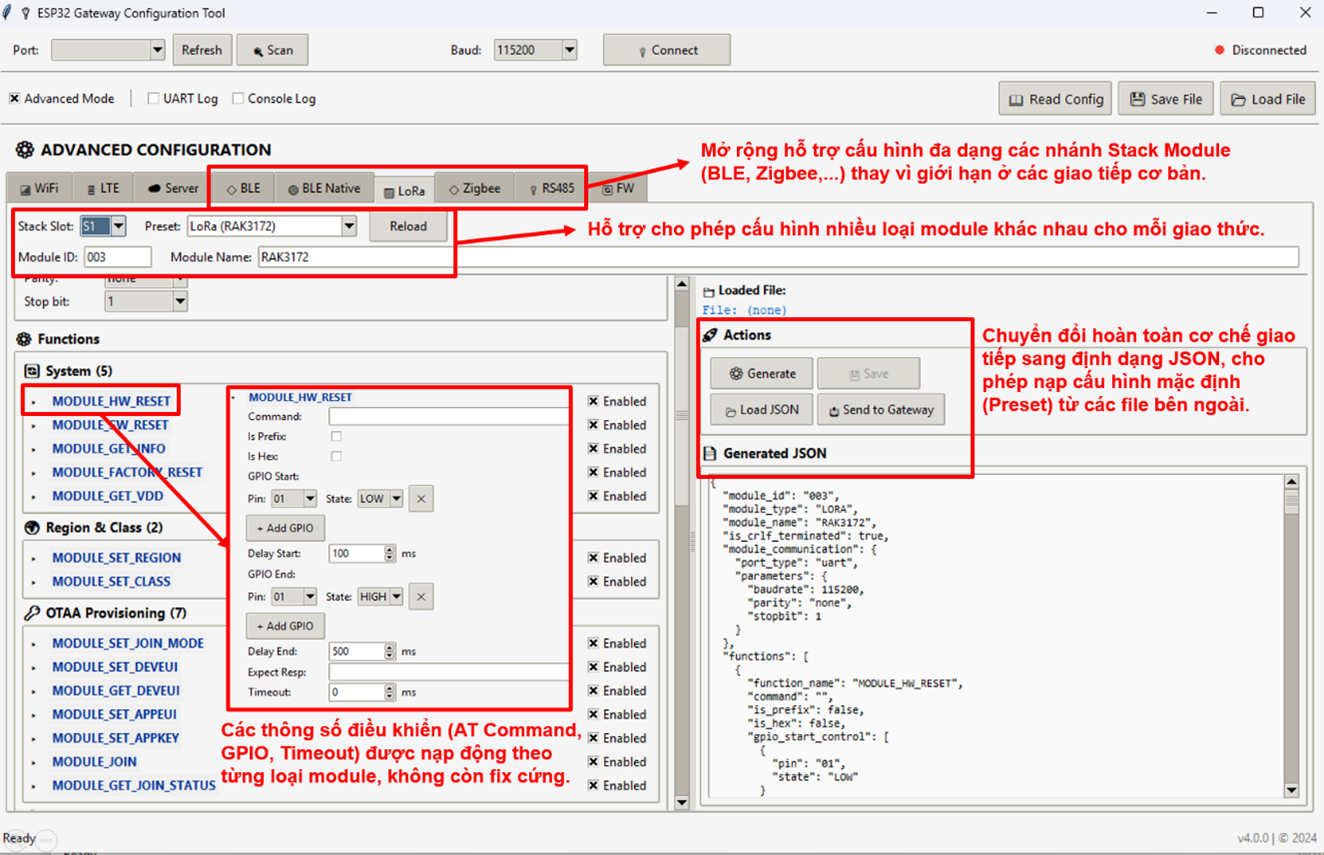
\includegraphics[width=\textwidth]{figures/giao_dien_pc_app2_ver_1_0_0.png}
            \caption{Logic cấu hình của phiên bản 1.0.0}
        \end{subfigure}
        \caption{So sánh logic cấu hình giữa phiên bản nguyên mẫu và phiên bản 1.0.0}
    \end{figure}

    Phần cấu hình server ở phiên bản 1.0.0 đã được chuẩn hóa cho đa giao thức (MQTT, HTTP/HTTPS, CoAP) thay vì chỉ tập trung vào MQTT như phiên bản nguyên mẫu, cho phép tùy chỉnh trực tiếp các tham số chuyên sâu như TLS, token và cơ chế truyền lại ngay trên giao diện. Đặc biệt, hệ thống bổ sung Web Config Portal chạy trực tiếp trên gateway, hỗ trợ mDNS và captive portal, đánh dấu bước chuyển quan trọng từ việc phụ thuộc vào kết nối máy tính qua cổng COM sang mô hình cấu hình không dây qua trình duyệt. Sự kết hợp giữa phần mềm desktop hoàn thiện và giao diện web trực tiếp giúp gateway đạt được sự tiện lợi và linh hoạt tối đa trong việc vận hành và giám sát trạng thái hệ thống.
    % \newpage
    \begin{figure}[h]
        \centering
        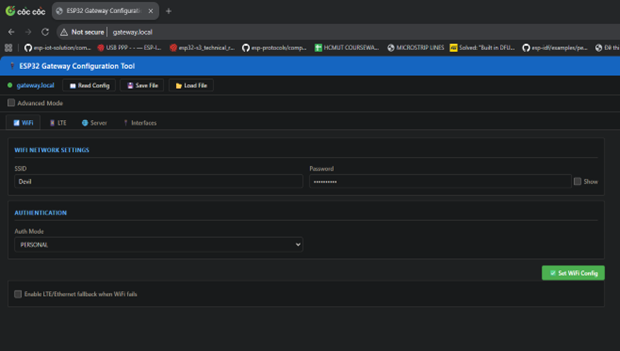
\includegraphics[width=0.9\textwidth]{figures/web_config_portal_ver_1_0_0.png}
        \caption{Giao diện Web Config Portal của phiên bản 1.0.0}
    \end{figure}
